%-------------------------------------------------------------------------------
% File:		Homework.tex
% Author:	Igor Janjic, Brian Hilnbrand, Danny Duangphachanh, Leah
%		Krynitsky  
% Description:	[ECE 4534] Embedded Systems Design
%		Background Research Assignment
%%------------------------------------------------------------------------------ 

%-------------------------------------------------------------------------------
% File:		Preamble.tex
% Author:	Igor Janjic
% Description:	Defines which packages to use.
%%------------------------------------------------------------------------------

\documentclass[11pt]{article}

% Encodes font as T1.
\usepackage[T1]{fontenc}

% Pretty much all of the ams maths packages.
\usepackage{amsmath,amsthm,amssymb,amsfonts}

% Allows you to manipulate the page a bit.
\usepackage[margin=0.75in]{geometry}

% Removes paragraph indentation.
\usepackage{parskip}

% Allows inclusion of graphics easily.
\usepackage{graphicx}

% Provides ways to make nice looking tables.
\usepackage{booktabs}

% Allows rotation of tables and figures.
\usepackage{rotating}

% Allows color.
\usepackage{color}

% Allows shading of table cells.
\usepackage{colortbl}

% Allows hyphenatable letterspacing, underlining, and highlighting.
\usepackage{soul}

% Allows extra text symbols.
\usepackage{textcomp}

% Allows manipulation of floats.
\usepackage{float}

% Provides commands to make subfigures.
\usepackage{subfigure}

% Typesets URLs sensibly with tt font, clickability in PDFs, and not breaking across lines.
\usepackage{url}

% Makes references hyperlinks in PDF output.
\usepackage{hyperref}

% Provides good access to colors.
\usepackage{color}

% Provides good access to colors.
\usepackage{xcolor}

% Provides for programming code to be inserted into the document.
\usepackage{listings}

% Provides support for table coloring.
\usepackage{xcolor}

% Provides vector graphics functionality.
\usepackage{tikz}
\usetikzlibrary{shapes.geometric, arrows, positioning}

% Provides circuit vector graphics functionality.
\usepackage{circuitikz}

% Provides caption manipulation.
\usepackage{caption}

% Makes sure tables don't float about if they have the designation [H].
\restylefloat{table}

% Defines the color gray.
\definecolor{gray}{rgb}{0.5, 0.5, 0.5}


%-------------------------------------------------------------------------------
% File:		Definitions.tex
% Author:	Igor Janjic
% Description:	Contains various commands.
%%------------------------------------------------------------------------------

%-------------------------------------------------------------------------------
% General Definitions

% Defines a command for skipping a line.
\def\wl{\par\vspace{\baselineskip}}

% Defines a command for hiding text.
\newcommand{\hide}[1]{}

% Defines a command for a shortened commonly used phrases.
\newcommand{\ie}{\text{i.e.}}
\newcommand{\eg}{\text{e.g.}}
\newcommand{\ex}{\text{e.x.}}
\newcommand{\ans}{\textbf{Answer: }}
\newcommand{\pro}{\textbf{Proof: }}

% Defines a command to mark to-do items in red.
\newcommand{\todo}[1] {\textbf{\textcolor{red}{#1}}}

% Defines commands for calligraphic font.
\newcommand{\calA}{\mathcal{A}}
\newcommand{\calB}{\mathcal{B}}
\newcommand{\calC}{\mathcal{C}}
\newcommand{\calD}{\mathcal{D}}
\newcommand{\calE}{\mathcal{E}}
\newcommand{\calF}{\mathcal{F}}
\newcommand{\calG}{\mathcal{G}}
\newcommand{\calH}{\mathcal{H}}
\newcommand{\calI}{\mathcal{I}}
\newcommand{\calJ}{\mathcal{J}}
\newcommand{\calK}{\mathcal{K}}
\newcommand{\calL}{\mathcal{L}}
\newcommand{\calM}{\mathcal{M}}
\newcommand{\calN}{\mathcal{N}}
\newcommand{\calO}{\mathcal{O}}
\newcommand{\calP}{\mathcal{P}}
\newcommand{\calQ}{\mathcal{Q}}
\newcommand{\calR}{\mathcal{R}}
\newcommand{\calS}{\mathcal{S}}
\newcommand{\calT}{\mathcal{T}}
\newcommand{\calU}{\mathcal{U}}
\newcommand{\calV}{\mathcal{V}}
\newcommand{\calW}{\mathcal{W}}
\newcommand{\calX}{\mathcal{X}}
\newcommand{\calY}{\mathcal{Y}}
\newcommand{\calZ}{\mathcal{Z}}

% Defines commands for bold font.
\newcommand{\bbA}{\mathbb{A}}
\newcommand{\bbB}{\mathbb{B}}
\newcommand{\bbC}{\mathbb{C}}
\newcommand{\bbD}{\mathbb{D}}
\newcommand{\bbE}{\mathbb{E}}
\newcommand{\bbF}{\mathbb{F}}
\newcommand{\bbG}{\mathbb{G}}
\newcommand{\bbH}{\mathbb{H}}
\newcommand{\bbI}{\mathbb{I}}
\newcommand{\bbJ}{\mathbb{J}}
\newcommand{\bbK}{\mathbb{K}}
\newcommand{\bbL}{\mathbb{L}}
\newcommand{\bbM}{\mathbb{M}}
\newcommand{\bbN}{\mathbb{N}}
\newcommand{\bbO}{\mathbb{O}}
\newcommand{\bbP}{\mathbb{P}}
\newcommand{\bbQ}{\mathbb{Q}}
\newcommand{\bbR}{\mathbb{R}}
\newcommand{\bbS}{\mathbb{S}}
\newcommand{\bbT}{\mathbb{T}}
\newcommand{\bbU}{\mathbb{U}}
\newcommand{\bbV}{\mathbb{V}}
\newcommand{\bbW}{\mathbb{W}}
\newcommand{\bbX}{\mathbb{X}}
\newcommand{\bbY}{\mathbb{Y}}
\newcommand{\bbZ}{\mathbb{Z}}

% Defines commands for bold face font.
\newcommand{\bfA}{\mathbf{A}}
\newcommand{\bfB}{\mathbf{B}}
\newcommand{\bfC}{\mathbf{C}}
\newcommand{\bfD}{\mathbf{D}}
\newcommand{\bfE}{\mathbf{E}}
\newcommand{\bfF}{\mathbf{F}}
\newcommand{\bfG}{\mathbf{G}}
\newcommand{\bfH}{\mathbf{H}}
\newcommand{\bfI}{\mathbf{I}}
\newcommand{\bfJ}{\mathbf{J}}
\newcommand{\bfK}{\mathbf{K}}
\newcommand{\bfL}{\mathbf{L}}
\newcommand{\bfM}{\mathbf{M}}
\newcommand{\bfN}{\mathbf{N}}
\newcommand{\bfO}{\mathbf{O}}
\newcommand{\bfP}{\mathbf{P}}
\newcommand{\bfQ}{\mathbf{Q}}
\newcommand{\bfR}{\mathbf{R}}
\newcommand{\bfS}{\mathbf{S}}
\newcommand{\bfT}{\mathbf{T}}
\newcommand{\bfU}{\mathbf{U}}
\newcommand{\bfV}{\mathbf{V}}
\newcommand{\bfW}{\mathbf{W}}
\newcommand{\bfX}{\mathbf{X}}
\newcommand{\bfY}{\mathbf{Y}}
\newcommand{\bfZ}{\mathbf{Z}}

% Defines commands for lists.
\newcommand{\be}{\begin{enumerate}}
\newcommand{\ee}{\end{enumerate}}
\newcommand{\ba}{\begin{align}}
\newcommand{\ea}{\end{align}}
\newcommand{\bas}{\begin{align*}}
\newcommand{\eassss}{\end{align*}}

%-------------------------------------------------------------------------------
% Math Definitions

% Defines a command for a function.
\newcommand{\func}[2]{#1 \left( #2 \right)}

% Defines a command for an integral.
\newcommand{\dint}[4]{\int_{#1}^{#2}#3\;d#4}

% Defines commands for objects.
\newcommand{\csum}[2]{\sum_{#1}^{#2}}
\newcommand{\cint}[2]{\int_{#1}{#2}}
\newcommand{\cprod}[2]{\prod_{#1}^{#2}}

% Defines commands for various parentheses.
\newcommand{\paren}[1]{\left( #1 \right)}
\newcommand{\sqprn}[1]{\left[ #1 \right]}
\newcommand{\tlprn}[1]{\left\{ #1 \right\}}

% Defines a command for the absolute value of an expression.
\newcommand{\abs}[1]{\left| #1 \right|}

% Defines commands for various angled expressions.
\newcommand{\tr}[2]{\left<\left< #1 , #2 \right>\right>}
\newcommand{\trs}[2]{\left< #1 , #2 \right>}
\newcommand{\iprod}[2]{\left\langle #1 , #2 \right\rangle}

% Defines commands for various deltas.
\newcommand{\del}{\partial}
\newcommand{\dd}[2]{\frac{d#1}{d#2}}
\newcommand{\ddel}[2]{\frac{\del#1}{\del#2}}
\newcommand{\ddell}[2]{\frac{\del^2#1}{{\del#2}^2}}
\newcommand{\ddelll}[3]{\frac{\del^2#1}{{\del#2}{\del#3}}}

% Defines a command for evaluating an expression at a particular value.
\newcommand{\eval}[3]{\left.#1\right|_{#2}^{#3}}

% Defines commands for flooring and ceiling.
\newcommand{\ceil}[1]{\ensuremath{\left\lceil#1\right\rceil}}
\newcommand{\floor}[1]{\ensuremath{\left\lfloor#1\right\rfloor}}

% Defines commands for argmin and argmax.
\newcommand{\argmin}{\mathop{\mathrm{argmin}}}
\newcommand{\argmax}{\mathop{\mathrm{argmax}}}

% Defines a command for mapping.
\newcommand{\map}{\mathop{\mathrm{map}}}

% Defines a command for an inverse.
\newcommand{\inv}{^{-1}}

% Defines a command for the partial derivative operator.
\newcommand{\pd}[2]{\frac{\partial #1}{\partial #2}}

% Defines commands for function names.
\newcommand{\zeros}{\mathrm{zeros}}
\newcommand{\rank}{\mathrm{rank}}
\newcommand{\TR}{\mathrm{tr}}
\newcommand{\vol}{\mathrm{vol}}
\newcommand{\sgn}{\mathrm{sgn}}
\newcommand{\acos}{\mathrm{acos}}
\newcommand{\intr}{\mathrm{int}\,}
\newcommand{\extr}{\mathrm{ext}\,}
\newcommand{\dom}{\mathrm{dom}\,}
\newcommand{\conv}{\mathrm{conv}\hspace{1pt}}
\newcommand{\cone}{\mathrm{cone}\hspace{1pt}}

% Defines commands for symbols in probability and statistics.
\newcommand{\convd}{\overset{{\scriptsize d}}{\to}}
\newcommand{\convp}{\overset{{\scriptsize p}}{\to}}
\newcommand{\unif}{\mathrm{Uniform}}
\newcommand{\bern}{\mathrm{Bernoulli}}
\newcommand{\negbin}{\mathrm{NegBinom}}
\newcommand{\Binom}{\mathrm{Bin}}
\newcommand{\pois}{\mathrm{Poisson}}
\newcommand{\ndistr}{\mathrm{n}}
\newcommand{\Bdistr}{\mathrm{Beta}}
\newcommand{\Gdistr}{\mathrm{Gamma}}
\newcommand{\iGdistr}{\mathrm{InvGamma}}
\newcommand{\MSE}{\mathrm{MSE}}
\newcommand{\MAE}{\mathrm{MAE}}
\newcommand{\ARE}{\mathrm{ARE}}
\newcommand{\se}{\mathrm{se}}
\newcommand{\mexp}{\text{{\bf E}}}
\newcommand{\var}{\mathrm{Var}}
\newcommand{\cov}{\mathrm{Cov}}
\newcommand{\corr}{\mathrm{Cor}}
\newcommand{\bW}{\bs{W}}
\newcommand{\bw}{\bs{w}}
\newcommand{\bX}{\bs{X}}
\newcommand{\bx}{\bs{x}}
\newcommand{\bY}{\bs{Y}}
\newcommand{\by}{\bs{y}}
\newcommand{\bZ}{\bs{Z}}
\newcommand{\bz}{\bs{z}}
\newcommand{\Xbar}{\overline{X}}
\newcommand{\ev}{\mathrm{Ev}}
\newcommand{\pr}{\boldsymbol{\mathrm{P}}}


%-------------------------------------------------------------------------------
% File:		Programming.tex
% Author:	Igor Janjic
% Description:	Defines programming environments.
%%------------------------------------------------------------------------------

\lstnewenvironment{matlab}{
\lstset{
    	language = matlab,	
	basicstyle = \footnotesize\ttfamily,
	numbers = left,
	numberstyle = \tiny\color{gray},
	stepnumber = 1,
	numbersep = 5pt,
 	backgroundcolor = \color{white},
 	showspaces = false,
  	showstringspaces = false,
  	showtabs = false,
  	frame = single,
  	rulecolor = \color{black},
  	tabsize = 4,
  	breaklines = true,
  	breakatwhitespace = false,
  	title = \lstname,
    	upquote = true,
    	aboveskip = {1.5\baselineskip},
    	columns=fixed,
   	extendedchars = true,
   	prebreak = \raisebox{0ex}[0ex][0ex]{\ensuremath{\hookleftarrow}},
    	identifierstyle=\ttfamily,
    	keywordstyle=\color[rgb]{0,0,1},
    	commentstyle=\color[rgb]{0.133,0.545,0.133},
    	stringstyle=\color[rgb]{0.627,0.126,0.941}
}}{}

\lstnewenvironment{tex}{
\lstset{
    	language = TeX,	
	basicstyle = \footnotesize\ttfamily,
	numbers = left,
	numberstyle = \tiny\color{gray},
	stepnumber = 1,
	numbersep = 5pt,
 	backgroundcolor = \color{white},
 	showspaces = false,
  	showstringspaces = false,
  	showtabs = false,
  	frame = shadowbox,
  	rulecolor = \color{black},
  	tabsize = 4,
  	breaklines = true,
  	breakatwhitespace = false,
  	title = \lstname,
    	upquote = true,
    	aboveskip = {1.5\baselineskip},
    	columns=fixed,
   	extendedchars = true,
    	identifierstyle=\ttfamily,
	xleftmargin=0.5cm,
	xrightmargin=0.5cm,
    	keywordstyle=\color[rgb]{0,0,1},
    	commentstyle=\color[rgb]{0.133,0.545,0.133},
    	stringstyle=\color[rgb]{0.627,0.126,0.941}
}}{}

\lstnewenvironment{pseudo}{
\lstset{
	basicstyle = \footnotesize,
	numbers = left,
	numberstyle = \tiny\color{gray},
	stepnumber = 1,
	numbersep = 5pt,
 	backgroundcolor = \color{white},
 	showspaces = false,
  	showstringspaces = false,
  	showtabs = false,
  	frame = single,
  	rulecolor = \color{black},
  	tabsize = 4,
  	captionpos = b,
  	breaklines = true,
  	breakatwhitespace = false,
  	title = \lstname,
    	upquote = true,
    	aboveskip = {1.5\baselineskip},
    	columns=fixed,
   	extendedchars = true,
   	prebreak = \raisebox{0ex}[0ex][0ex]{\ensuremath{\hookleftarrow}},
}}{}



\begin{document}

%-------------------------------------------------------------------------------
% File:		    Title.tex
% Author:	    Igor Janjic
% Description:	[ECE 4564] Network Applications Design
%		        Project proposal.
%%------------------------------------------------------------------------------

\begin{titlepage}

\centering
\vspace*{\baselineskip}

\rule{\textwidth}{1.6pt}\vspace*{-\baselineskip}\vspace*{2pt}
\rule{\textwidth}{0.4pt}\\[\baselineskip]

{\LARGE Final Report\\[0.3\baselineskip]}

\rule{\textwidth}{0.4pt}\vspace*{-\baselineskip}\vspace{3.2pt}
\rule{\textwidth}{1.6pt}\\[\baselineskip]

\wl

\scshape Due December 12, 2014 at 11:55 PM.
{\small 
\\[\baselineskip]\par}

\vfill

Created by:\\[0.2\baselineskip]
{Brian Hilnbrand:     \texttt{brhiln@vt.edu}}\\[0.2\baselineskip]
{Danny Duangphachanh: \texttt{bboydd@vt.edu}}\\[0.2\baselineskip]
{Igor Janjic:         \texttt{ijanjic@vt.edu}}\\[0.2\baselineskip]
{Leah Krynitsky:      \texttt{leah8@vt.edu}}\\[0.4\baselineskip]
{\small \today}\\[0.8\baselineskip]
{\small [ECE 4534] Embedded Systems Design}\\[0.2\baselineskip]
{\small\itshape Virginia Polytechnic Institute and\\ State University}\\[0.2\baselineskip]

\begin{center}
	
\includegraphics[scale=0.35]{Images/Logo}
\end{center}

\end{titlepage}


\subsection*{ARM Task Diagram}
The following is the task diagram for the ARM board.
\begin{center}
	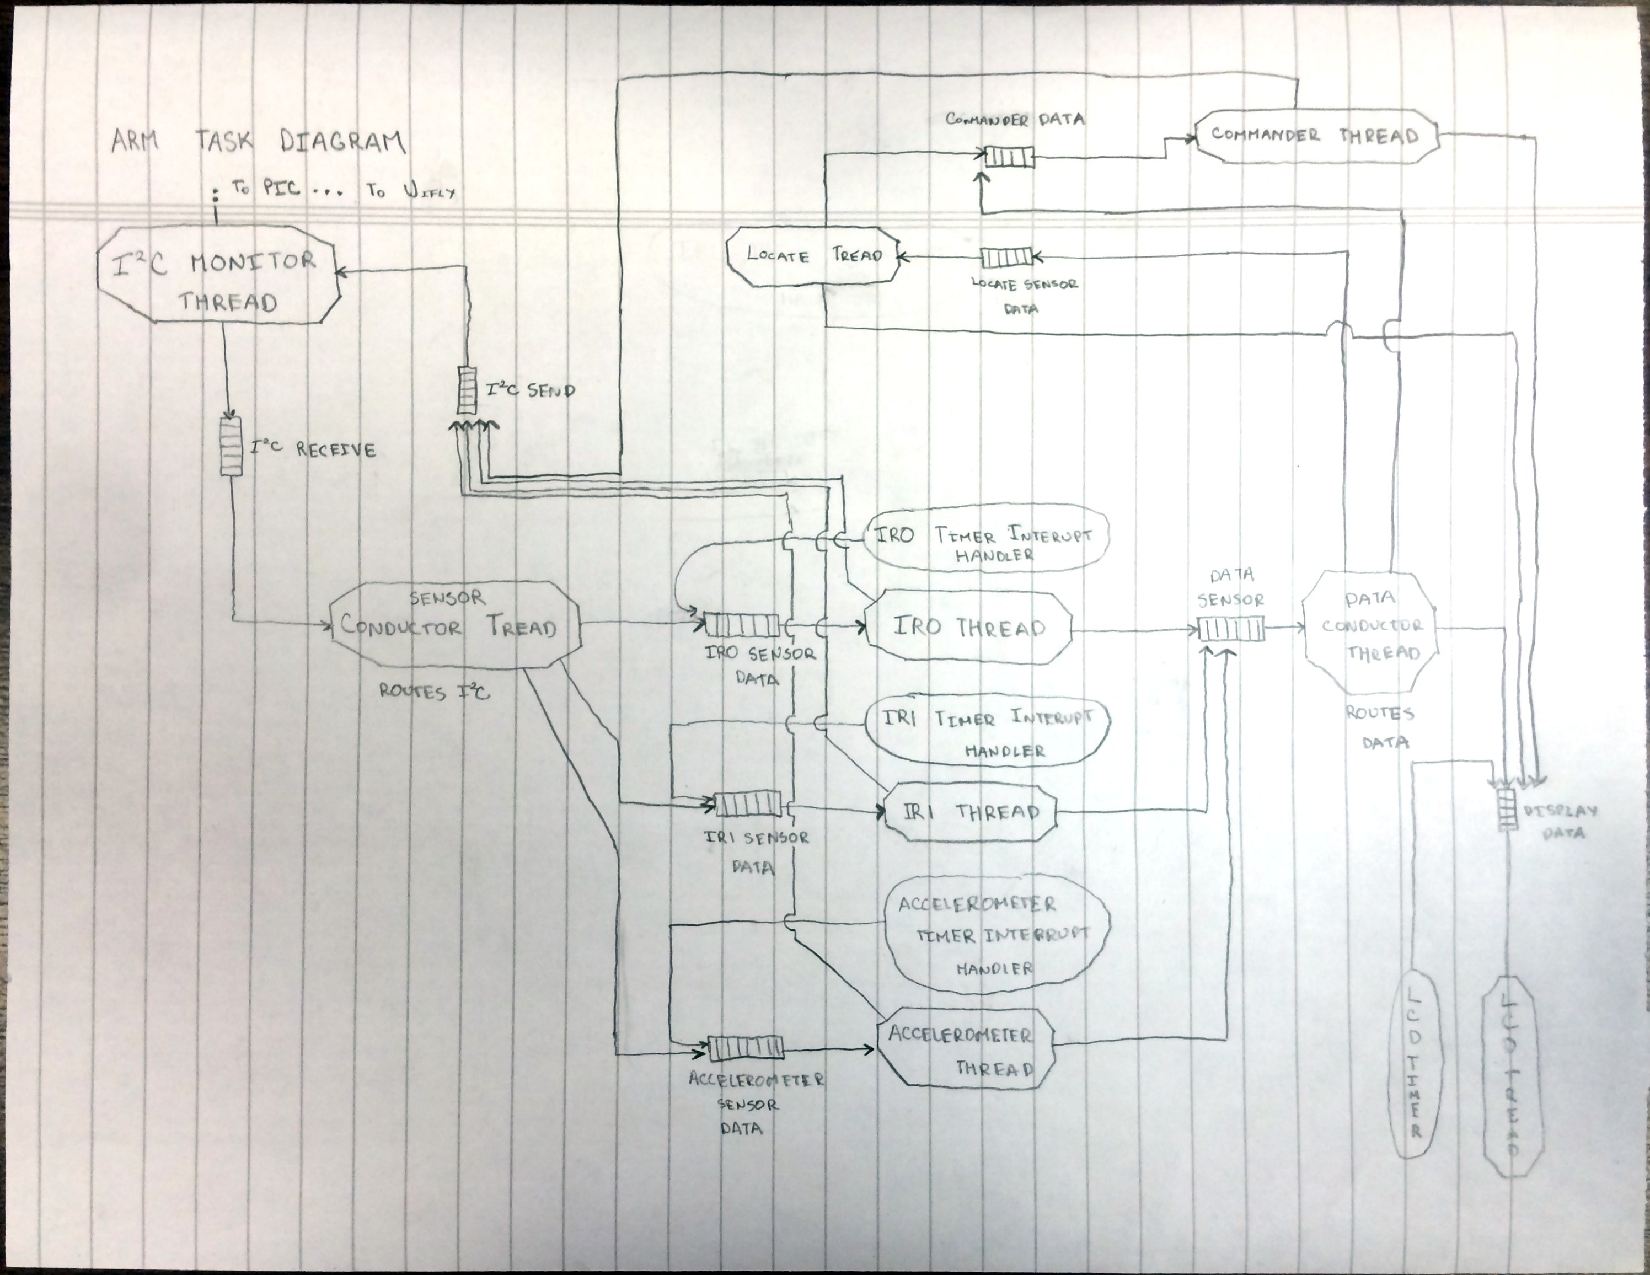
\includegraphics[scale=0.5]{Images/ARMTaskDiagram}
\end{center}

% Monitor Thread
\paragraph*{I$^2$C Monitor Thread}
\begin{enumerate}
	\item This thread handles all I$^2$C communications.
	\item Implemented in \texttt{vtI2C.c}.
	\item Queue: I$^2$C Receive
	\begin{enumerate}
		\item This queue contains received messages via I$^2$C and sends them to the Sensor Conductor Thread.
		\item The received messages will have varying formats depending on the sensors that sent them. These formats will be described in the description for the sensor task diagram.
	\end{enumerate}
	\item Queue: I$^2$C Send
	\begin{enumerate}
		\item This queue contains sent messages via I$^2$C to the master PIC.
		\item The sent messages will have varying formats depending on the threads that send them.
	\end{enumerate}
\end{enumerate}

% Conductor Thread
\paragraph*{Sensor Conductor Thread}
\begin{enumerate}
	\item This thread routes received I$^2$C data and sends it to the various sensor threads.
	\item Implemented in \texttt{sensorConductor.c}.
\end{enumerate}

% IR0 Thread
\paragraph*{IR0 Thread}
\begin{enumerate}
	\item This thread processes received IR0 sensor data and sends it to the Data Conductor Thread.
	\item Implemented in \texttt{i2cIRO.c}.
	\item This thread has a timer interrupt handler.
	\item Queue: IRO Sensor Data
	\begin{enumerate}
		\item This queue contains IR0 sensor data received via I$^2$C as well as data from the interrupt handler for this thread.
		\item The received data will have type \texttt{unsigned int} and will represent the voltage of the IR0 sensor.
	\end{enumerate}
\end{enumerate}

% IR1 Thread
\paragraph*{IR1 Thread}
\begin{enumerate}
	\item This thread processes received IR1 sensor data and sends it to the Data Conductor Thread.
	\item Implemented in \texttt{i2cIR1.c}.
	\item This thread has a timer interrupt handler.
	\item Queue: IR1 Sensor Data
	\begin{enumerate}
		\item This queue contains IR1 sensor data received via I$^2$C as well as data from the interrupt handler for this thread.
		\item The received data will have type \texttt{unsigned int} and will represent the voltage of the IR1 sensor.
	\end{enumerate}
\end{enumerate}

% Accelerometer Thread
\paragraph*{Accelerometer Thread}
\begin{enumerate}
	\item This thread processes received accelerometer sensor data and sends it to the Data Conductor Thread.
	\item Implemented in \texttt{i2cAccel.c}.
	\item This thread has a timer interrupt handler.
	\item Queue: Accelerometer Sensor Data
	\begin{enumerate}
		\item This queue contains accelerometer sensor data received via I$^2$C as well as data from the interrupt handler for this thread.
		\item The received data will have type \texttt{int} and will represent the voltage of the accelerometer sensor.
	\end{enumerate}
\end{enumerate}

% Data Conductor Thread
\paragraph*{Data Conductor Thread}
\begin{enumerate}
	\item This thread routes received sensor data from each sensor thread and sends it to a variety of processing threads. Relevant data is sent to the Locate Thread and LCD Thread.
	\item Implemented in \texttt{dataConductor.c}.
	\item Queue: Data Sensor
	\begin{enumerate}
		\item This queue contains all preprocessed sensor data.
		\item The received data will have various types explained in each relevant sensor thread description.
	\end{enumerate}
\end{enumerate}

% LCD Thread
\paragraph*{LCD Thread}
\begin{enumerate}
	\item This thread displays the following on the LCD: raw sensor data (Data Conductor Thread), location data (Locate Thread), commands being sent to the motor controller (Command Thread).
	\item Implemented in \texttt{LCDtask.c}.
	\item This thread has a timer interrupt handler.
	\item Queue: Display Data
	\begin{enumerate}
		\item This queue contains all data that will be displayed.
		\item The received data will have various types explained in each relevant thread.
	\end{enumerate}
\end{enumerate}

% Locate Thread
\paragraph*{Locate Thread}
\begin{enumerate}
	\item This thread processes all relevant sensor data (IR0 and IR1) and determines the location of the rover which it then sends to the Commander Thread.
	\item Implemented in \texttt{locateTask.c}.
	\item Queue: Locate Sensor Data
	\begin{enumerate}
		\item This queue contains all sensor data used to find the location of the rover.
		\item The received data will have various types explained in each relevant thread.
	\end{enumerate}
\end{enumerate}

% Commander Thread
\paragraph*{Commander Thread}
\begin{enumerate}
	\item This thread processes the location and determines the next motor movement which it then sends to the I$^2$ Moniter Thread (ultimately sending the command to the Motor PIC.
	\item Implemented in \texttt{commanderTask.c}.
	\item Queue: Commander Data
	\begin{enumerate}
		\item This queue contains all sensor data used to determine the next movement of the rover.
		\item The received data will have various types explained in each relevant thread.
	\end{enumerate}
\end{enumerate}

\subsection*{Slave Task Diagram}

\begin{center}
	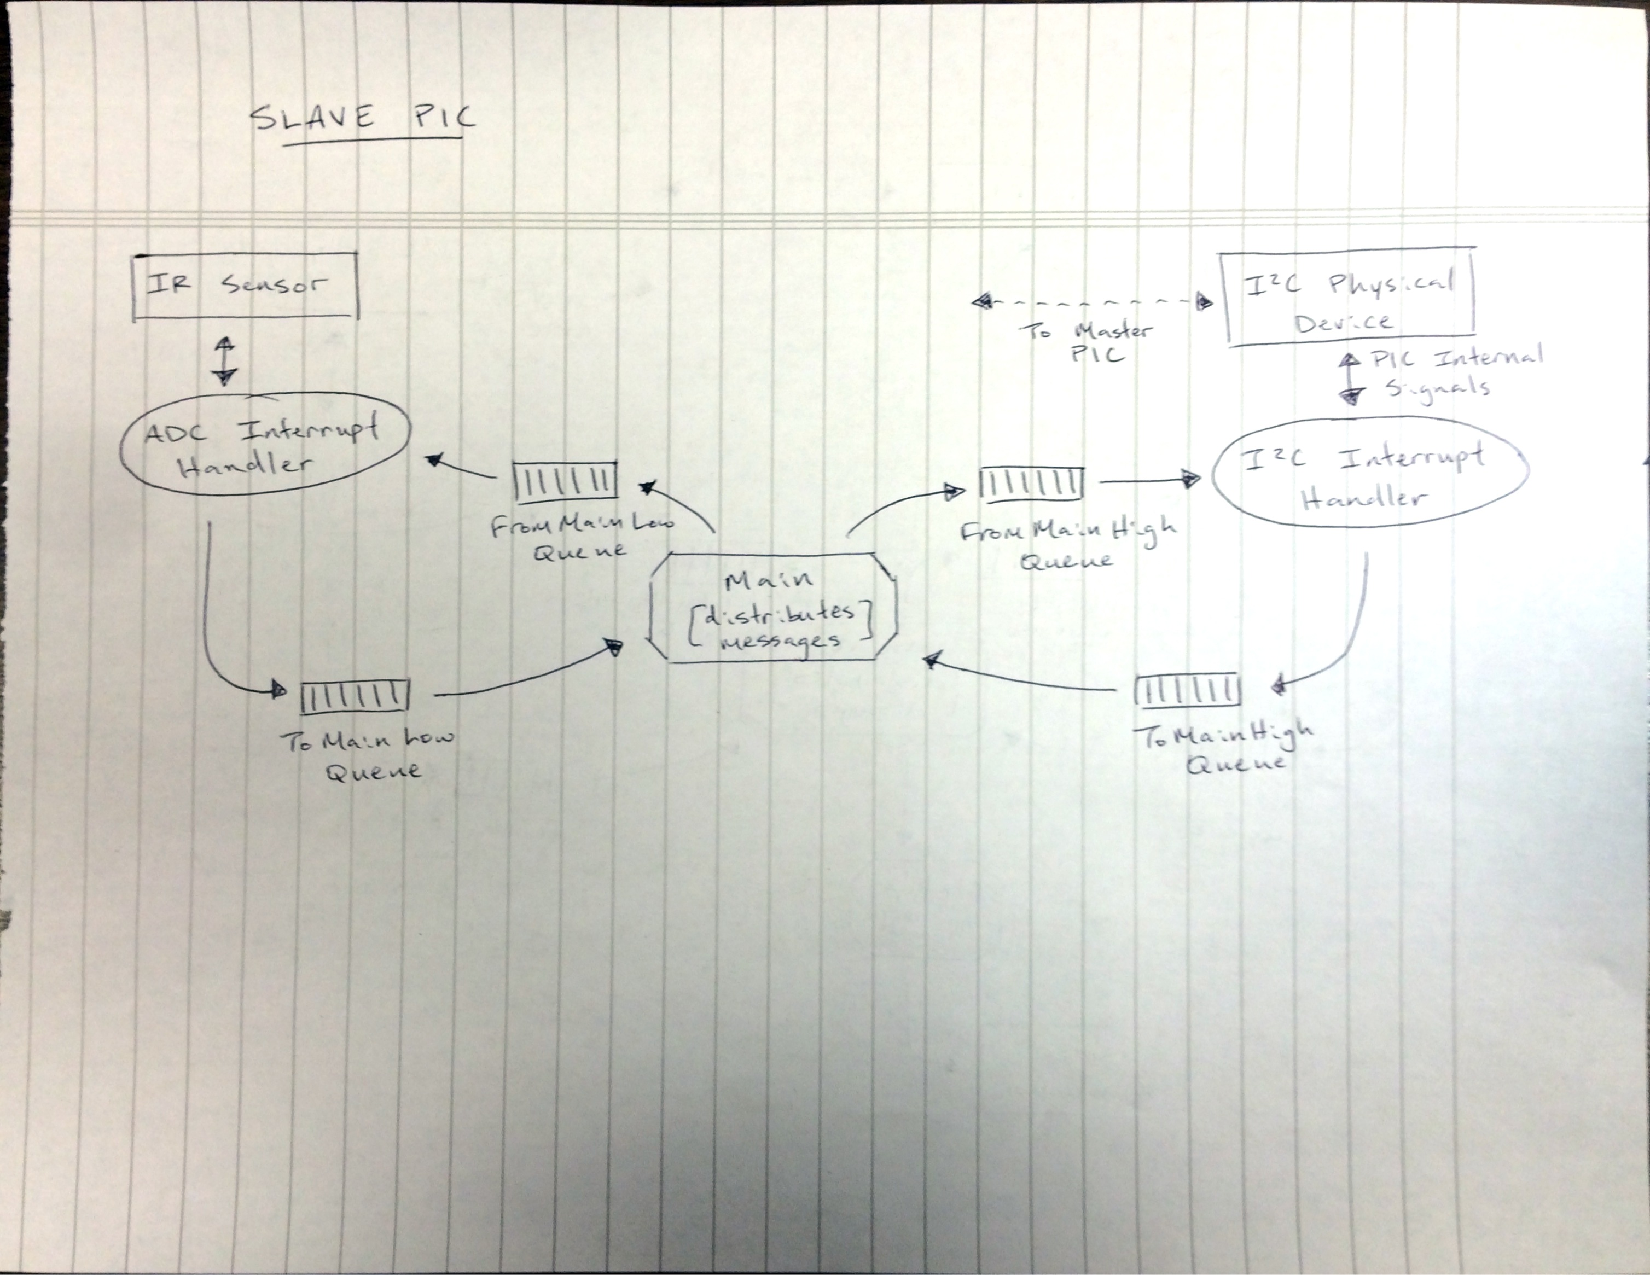
\includegraphics[scale=0.45]{Images/SlaveTaskDiagram}
\end{center}

\subsection*{Master Task Diagram}

\begin{center}
	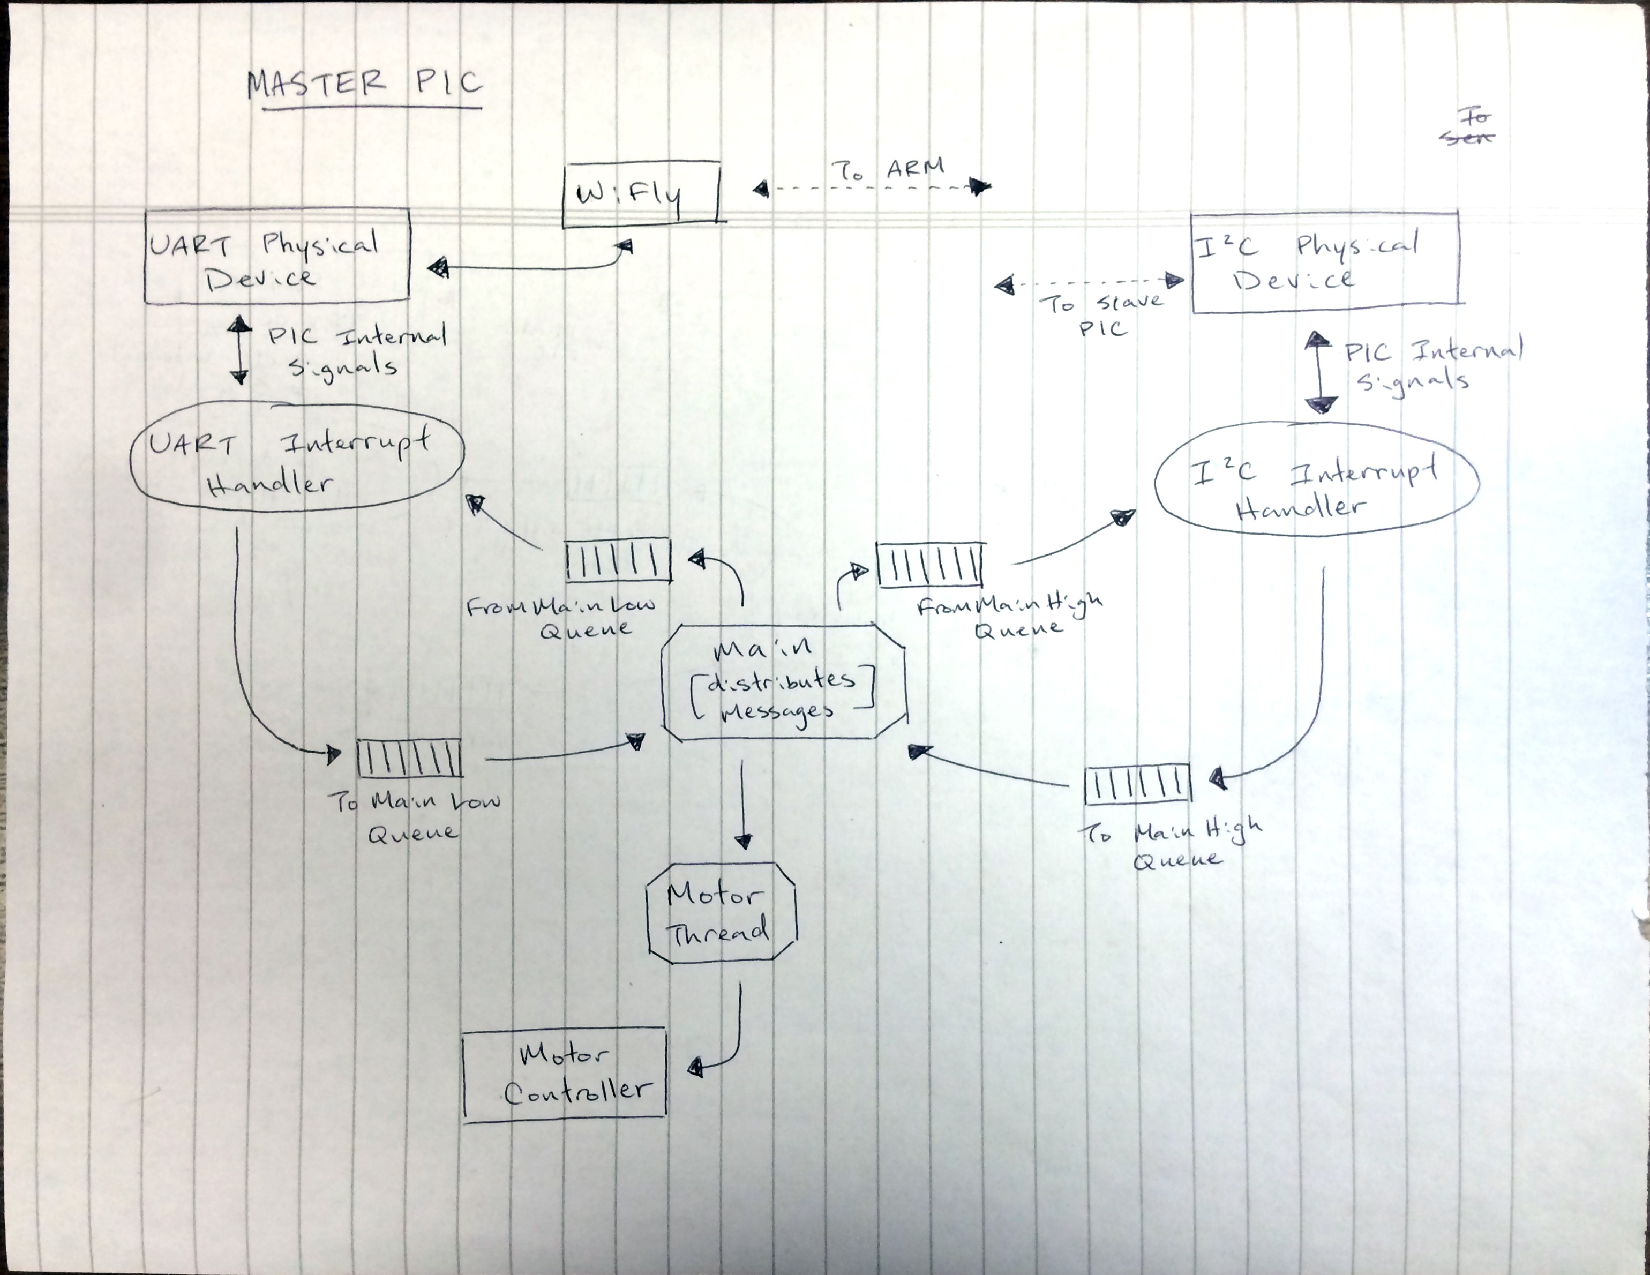
\includegraphics[scale=0.45]{Images/MasterTaskDiagram}
\end{center}

\paragraph*{Main Thread}


Distributes the message passing between MainLow and MainHigh queues and also handles initiation of all devices, threads, and interrupt handlers. 

\paragraph*{Motor Thread}\mbox{}\\
Receives signals from Main. Communicates with the Motor Controller.

\paragraph*{UART Interrupt Handler}\mbox{}\\
Interrupts whenever the UART Physical Device is ready to send or receive a message. 

\paragraph*{I$^2$C Interrupt Handler}\mbox{}\\
Interrupts whenever the I2C Physical Device is ready to send or receive a message to the other PIC. 

\paragraph*{ADC Interrupt Handler}\mbox{}\\
Interrupts whenever the ADC is ready to initiate read or receive.

\paragraph*{WiFly Physical Device}\mbox{}\\
Wireless transmitter/receiver.

\paragraph*{UART Physical Device}\mbox{}\\
Communicates with the WiFly. 

\paragraph*{I$^2$C Physical Device}\mbox{}\\
Communicates with the other I2C Physical Device to communicate with the other PIC. 

\paragraph*{Motor Controller Physical Device}\mbox{}\\
Sends power to the motors. 

\paragraph*{IR Sensors Physical Devices}\mbox{}\\
Reads the area directly in front of the sensor area.

\paragraph*{ToMainHigh Message Queue}\mbox{}\\
Handles messages from the I2C Physical Device to Main. 

\paragraph*{FromMainHigh Message Queue}\mbox{}\\
Handles messages from Main to to I2C Physical Device. 

\paragraph*{ToMainLow Message Queue}\mbox{}\\
Handles messages from the UART and IR Sensor on the Master and Slave PIC, respectively.

\paragraph*{FromMainLow Message Queue}\mbox{}\\
Handles messages from Main to the UART and IR Sensor on the Master and Slave PIC, respectively.

\end{document}
